\chapter{Water flow module}

\section{Infiltration- Part 1}
\subsection{Goal and Complexity}
\subsubsection*{Complexity: Beginner}

\subsubsection*{Prerequisites: None}

The goal of this tutorial is to get familiar with the $DRUtES$ standard Richards equation module and $DRUtES$ configuration in 1D by simulating infiltration into different soil \medskip

\begin{figure}[!h]
\centering
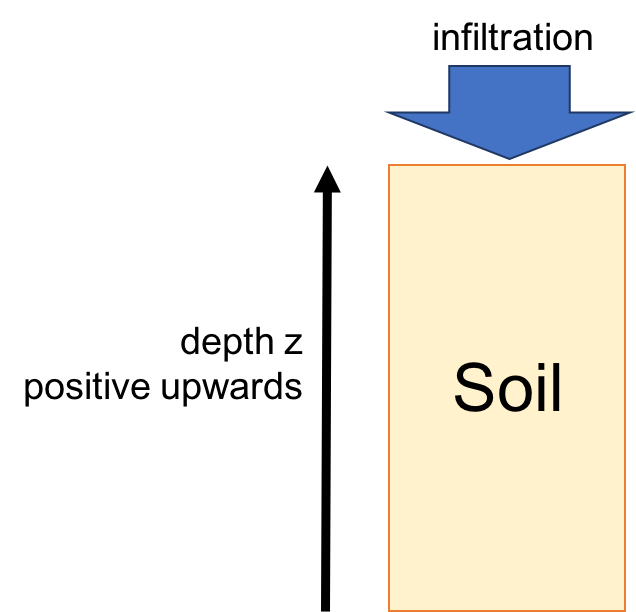
\includegraphics[width=8cm]{Fig_inf1/infilt.png}
\end{figure}
The process of infiltration is fundamental and yet very important in soil science. Infiltration into the soil determines water, heat and contaminant transport. Infiltration experiments can be used to determine some parameters describing soil hydraulic properties. 

In this tutorial three configuration files will be modified step by step. All configuration files are located in the folder \emph{drutes.conf} and respective subfolders. \begin{enumerate}
\item For selection of the module, dimension and time information we require \emph{global.conf}.  \emph{global.conf} is located in \emph{drutes.conf / global.conf}. 
\item To define the mesh or spatial discretization in 1D,  we require \emph{drumesh1D.conf}. \emph{drumesh1D.conf} is located in \emph{drutes.conf / mesh / drumesh1D.conf}. 
\item To define the infiltration, we require \emph{matrix.conf}. \emph{matrix.conf} is located in \emph{drutes.conf /water.conf/ matrix.conf}. 
\end{enumerate}
$DRUtES$ works with configuration input file with the file extension .conf. Blank lines and lines starting with \# are ignored. The input mentioned in this tutorial therefore needs to be placed one line below the mentioned keyword, unless stated otherwise. 

\newpage
\subsection{Scenarios}

We are using the well-known van Genuchten-Mualem parameterization to describe the soil hydraulic properties of our soils. 

\begin{table}[!h]
\centering
\caption{\label{tab_heat}Material properties needed for scenarios.}
\adjustbox{max height=\dimexpr\textheight-2cm\relax,
           max width=\textwidth}{

\small\begin{tabular}{l l c c c c c c}
\hline
Parameter & Description & Sand & Silt & Clay\\
\hline

$\alpha$ [cm$^{-1}$]& inverse of the air entry value &0.10 &0.08&0.01 \\
 $n$ [-]& shape parameter &2.2  & 1.8&1.5  \\
 $m$ [-]& shape parameter &0.55  & 0.44 & 0.33  \\
  $ \theta_s$ [-]&saturated vol. water content&0.4  & 0.45 & 0.5  \\
  $ \theta_r$ [-]& residual vol. water content&0.0 & 0.05 & 0.1  \\
  $Ss$ [cm$^{-1}$] & specific storage & 1e-9 & 1e-9 & 1e-10 \\
  $K_s$ [cm d$^{-1}$] & saturated hydraulic conductivity & 400 & 40 & 4 \\ 
\hline
\end{tabular}
}
\end{table}
\begin{figure}[!h]

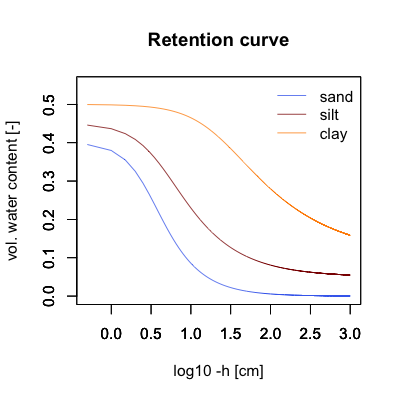
\includegraphics[width=6cm]{Fig_inf1/retention_curve.png}
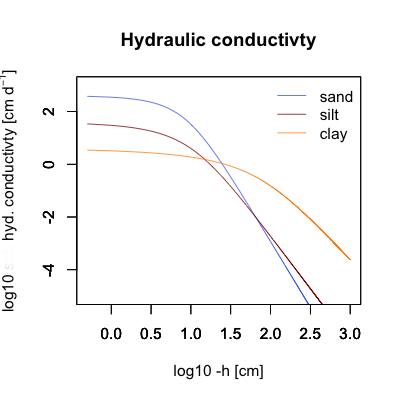
\includegraphics[width=6cm]{Fig_inf1/cond_hyd_curve.png}
\end{figure}

\section*{Scenario 1}

Infiltration into sandy soil. 

$global.conf$: Choose correct model, dimension, time discretization and observation times.
\begin{enumerate}
\item Open \textbf{\emph{global.conf}} in a text editor of your choice. 
\item Model type: Your first input is the module. Input is \textbf{RE}.
\item Initial mesh configuration \begin{enumerate}
\item The dimension of our problem is 1. Input: 1.
\item We use the internal mesh generator. Input: 1.
\end{enumerate}
\item Error criterion \begin{enumerate} 
\item Maximum number of iteration of the Picard method: 20.
\item h tolerance: 1e-1.
\end{enumerate}
\item Time information 
\begin{enumerate} 
%\item integration method is 3 point formula. Input: 30. 
\item Time units are in hours: input d.
\item Initial time: 1e-4.
\item End time: 1.
\item Minimum time step: 1e-4.
\item Maximum time step: 0.1.
\end{enumerate}
\item Observation time settings \begin{enumerate}
\item Observation time method: 2.
\item Set file format of observation: pure. Output in 1D is always in raw data. Different options will not impact output in 1D.
\item Make sequence of observation time: n.
\item Number of observation times: 10.
\item Observation time values: 0.001,
0.005,
0.01,
0.05,
0.1,
0.2,
0.3,
0.4,
0.6,
0.8. Use a new line for each input. \textit{DRUtES} automatically generates output for the initial time and final time. DRUtES will generate 12 output files, e.g. \textit{RE\_matrix\_press\_head-x.dat}, \textit{RE\_matrix\_theta-x.dat} where x is the number of the file and not the output time. The initial time is assigned an x value of 0. 
\end{enumerate}
\item Observation point settings \begin{enumerate}
\item Observation point coordinates: 0, 200. Use a new line for each input. \textit{DRUtES} will generate 2 output files, e.g. \textit{obspt\_RE\_matrix-1.out}, where x is the ID of the observation point. 
\end{enumerate}
\item Ignore other settings for now. 
\item Save $global.conf$
\end{enumerate}


$drumesh1D.conf$: Mesh definition, i.e. number of materials and spatial discretization
\begin{enumerate}
\item Open \textbf{\emph{drumesh1D.conf}} in a text editor of your choice. 
\item Geometry information: 200 cm - domain length
\item Amount of intervals: 1
\item
\adjustbox{max height=\dimexpr\textheight-5cm\relax,
           max width=\textwidth}{
\small\begin{tabular}{|c | c | c|}
\hline
density & bottom & top \\
 \hline
5 & 0 & 200\\
\hline
\end{tabular}
}
\item Number of materials: 1
\item \adjustbox{max height=\dimexpr\textheight-5cm\relax,
           max width=\textwidth}{
\small\begin{tabular}{|c | c | c|}
\hline
id & bottom & top \\
 \hline
5 & 0 & 200 \\
\hline
\end{tabular}
}
\end{enumerate}

\emph{matrix.conf}: Configuration file for water flow 


\begin{enumerate}
\item Open \emph{matrix.conf} in a text editor of your choice. 
\item How-to use constitutive relations? [integer]: 1
\item Length of interval for precalculating the constitutive functions: 200
\item Discretization step for constituitive function precalculation: 0.1
\item Number of soil layers [integer]: 1
\item \adjustbox{max height=\dimexpr\textheight-5cm\relax,
	max width=\textwidth}{
	\small\begin{tabular}{|c | c | c|c | c | c|}
		\hline
		alpha & n & m & theta\_r & theta\_s & specific storage\\
		\hline
		0.1 & 2.2  & 0.55 & 0.00 & 0.40  &1e-9  \\
		\hline
	\end{tabular}
}
\item The angle of the anistropy determines the angle of the reference coordinate system. 0 means vertical flow. Anisothpropy description. Anisothpropy description and hydraulic conductivity\\ \adjustbox{max height=\dimexpr\textheight-5cm\relax,
	max width=\textwidth}{
	\small\begin{tabular}{|c | c |}
		\hline
		angle [degrees] & K\_11  \\
		\hline
		0 & 400  \\
		\hline
	\end{tabular}
}
\item sink(-) /source (+) term per layer: 0
\item \adjustbox{max height=\dimexpr\textheight-5cm\relax,
	max width=\textwidth}{
	\small\begin{tabular}{|c | c | c|c |}
		\hline
		 init. cond [real] & type of init. cond &RCZA method [y/n] &  RCZA method val.  \\
		\hline
		   0.0           &            H\_tot                       & n		   &          0 \\
		\hline
	\end{tabular}
}
\item number of boundaries: 2
\item \adjustbox{max height=\dimexpr\textheight-5cm\relax,
	max width=\textwidth}{
	\small\begin{tabular}{|c | c | c|c |}
		\hline
		boundary ID& boundary type   & use rain.dat [y/n]   & value  \\
		\hline
	101    &                   1        &           n        &        0.0 \\
	102             &          2         &          n         &       4        \\
	
		\hline
	\end{tabular}
}
\item Save matrix.conf.

\end{enumerate}

\subsection*{Run scenario 1}
Run the simulation in the terminal console.
\begin{enumerate}
\item Make sure you are in the right directory. 
\item To execute $DRUtES$: \\
\$ bin/drutes
\item After the simulation finishes, to generate png plots execute provided R script: \\
\$ Rscript drutes.conf/water.conf/waterplots.R -name sand
\item The output of the simulation can be found in the folder out
\end{enumerate}

\subsection*{Scenario 2}
Infiltration into silty soil
\begin{enumerate}
\item \emph{global.conf} and \emph{drumesh1D.conf} remain the same.
\item Open \emph{matrix.conf} in a text editor of your choice. 
\item Use the same set-up, but change the van Genuchten parameters to:
\item \adjustbox{max height=\dimexpr\textheight-5cm\relax,
	max width=\textwidth}{
	\small\begin{tabular}{|c | c | c|c | c | c|}
		\hline
		alpha & n & m & theta\_r & theta\_s & specific storage\\
		\hline
		0.08 & 1.8   & 0.44 & 0.05 & 0.45  & 1e-9 \\
		\hline
	\end{tabular}
}
\item anisothprophy description and hydraulic conductivity\\ \adjustbox{max height=\dimexpr\textheight-5cm\relax,
	max width=\textwidth}{
	\small\begin{tabular}{|c | c |}
		\hline
		angle [degrees] & K\_11  \\
		\hline
		0 & 40  \\
		\hline
	\end{tabular}
}
\item Save matrix.conf.
\end{enumerate}

\subsection*{Run scenario 2}
Run the simulation in the terminal console.
\begin{enumerate}
\item To execute $DRUtES$: \\
\$ bin/drutes
\item generate png plots with R script: \\
\$ Rscript drutes.conf/water.conf/waterplots.R -name silt
\end{enumerate}

\subsection*{Scenario 3}
Infiltration into clay soil
\begin{enumerate}
\item \emph{global.conf} and \emph{drumesh1D.conf} remain the same.
\item Open \emph{matrix.conf} in a text editor of your choice. 
\item Use the same set-up, but change the van Genuchten parameters to:
\item \adjustbox{max height=\dimexpr\textheight-5cm\relax,
	max width=\textwidth}{
	\small\begin{tabular}{|c | c | c|c | c | c|}
		\hline
		alpha & n & m & theta\_r & theta\_s & specific storage\\
		\hline
		0.01 & 1.5  & 0.33 & 0.1& 0.5   &1e-10 \\
		\hline
	\end{tabular}
}
\item anisothprophy description and hydraulic conductivity\\ \adjustbox{max height=\dimexpr\textheight-5cm\relax,
	max width=\textwidth}{
	\small\begin{tabular}{|c | c |}
		\hline
		angle [degrees] & K\_11  \\
		\hline
		0 & 4  \\
		\hline
	\end{tabular}
}
\item Save matrix.conf.
\end{enumerate}

\subsection*{Run scenario 3}
Run the simulation in the terminal console.
\begin{enumerate}
\item To execute $DRUtES$: \\
\$ bin/drutes
\item generate png plots with R script: \\
\$ Rscript drutes.conf/water.conf/waterplots.R -name clay
\end{enumerate}

\subsection*{Tasks}

\begin{enumerate}
\item Describe the infiltration fronts for sand, silt and clay.
\item The results of the fluxes look horrible. This is because of insufficient discretization. Improve the discretization. With what set-up are the results better? Possibilities are: 
\begin{itemize}
\item in global.conf: Decrease the pressure head tolerance, Decrease the initial time step, Decrease the maximum time step.
\item in drumesh1D.conf: Decrease the mesh density. 
\end{itemize}
\end{enumerate}



\subsection*{Results}
In the following time series of the infiltration into sand, silt and clay are presented. The infiltration front has moved furthest in clay, followed by sand and then silt. However, the time series show that their numerical approximation is insufficient, especially for sand. This is because sand is the numerically most difficult to model as it has the steepest retention properties (largest n and largest alpha). In the beginning, the flux in sand is 100 cm d$^{-1}$, which is 20 times the size of the assigned flux. For silt, the flux is overestimated approximately 12 times and for clay, the flux is overestimated twice. 

\begin{figure}
\centering
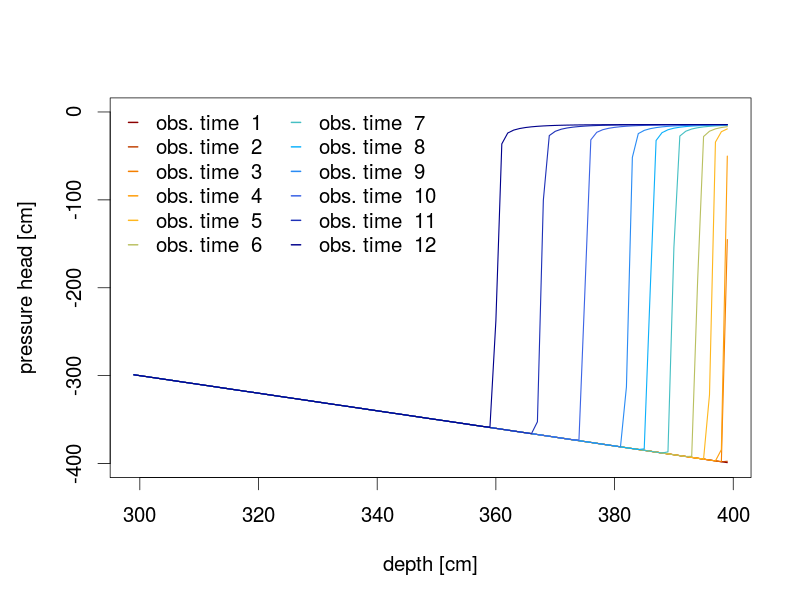
\includegraphics[width=0.49\textwidth]{Fig_inf1/obs_press_head_sand.png}
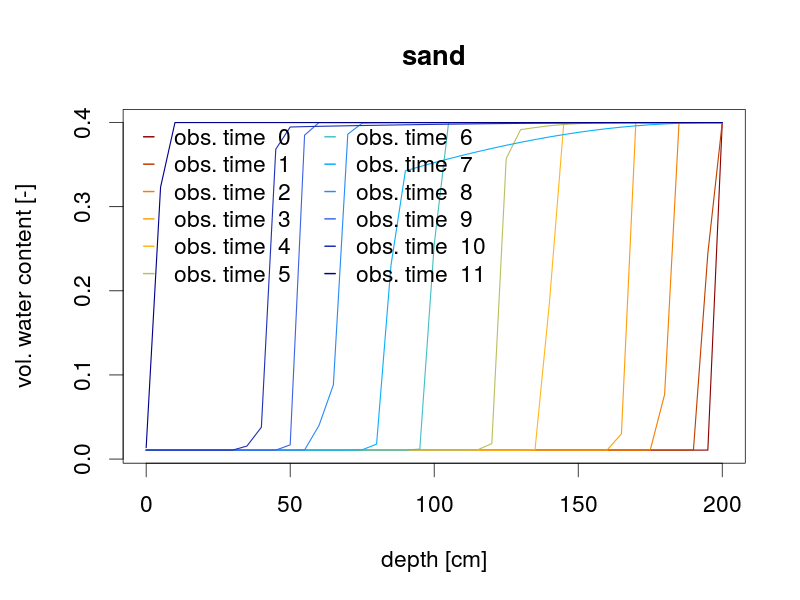
\includegraphics[width=0.49\textwidth]{Fig_inf1/obs_water_sand.png}
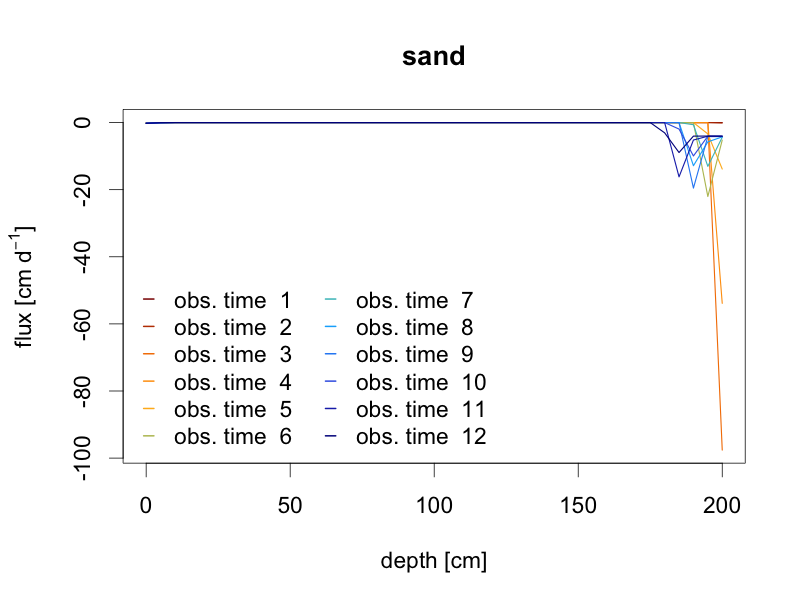
\includegraphics[width=0.49\textwidth]{Fig_inf1/obs_flux_sand.png}
\caption{Observation time series of pressure head, vol. water content and flux of infiltration into sand.}
\end{figure}

\begin{figure}
\centering
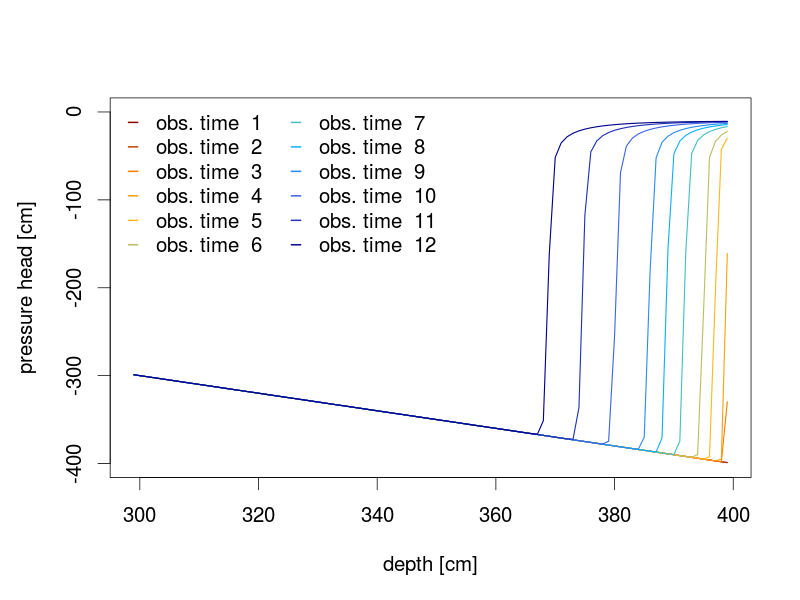
\includegraphics[width=0.49\textwidth]{Fig_inf1/obs_press_head_silt.png}
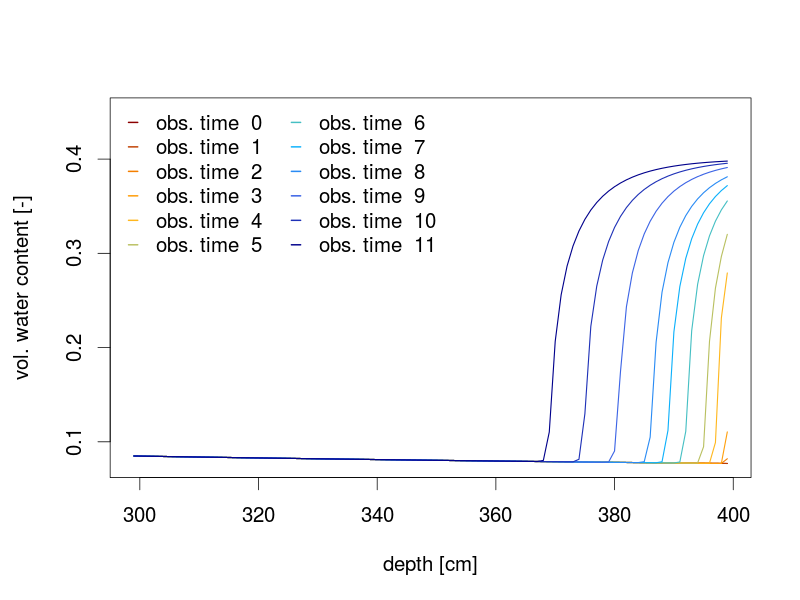
\includegraphics[width=0.49\textwidth]{Fig_inf1/obs_water_silt.png}
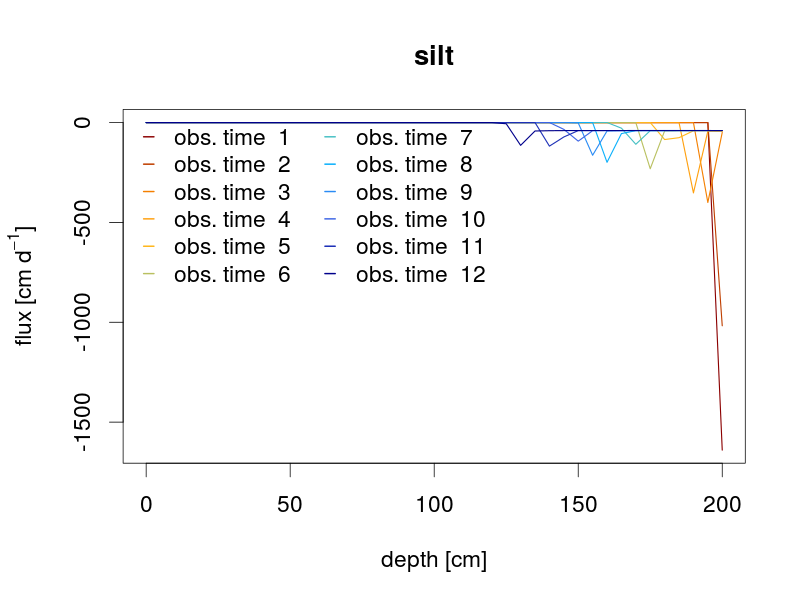
\includegraphics[width=0.49\textwidth]{Fig_inf1/obs_flux_silt.png}
\caption{Observation time series of pressure head, vol. water content and flux of infiltration into silt.}

\end{figure}


\begin{figure}
\centering
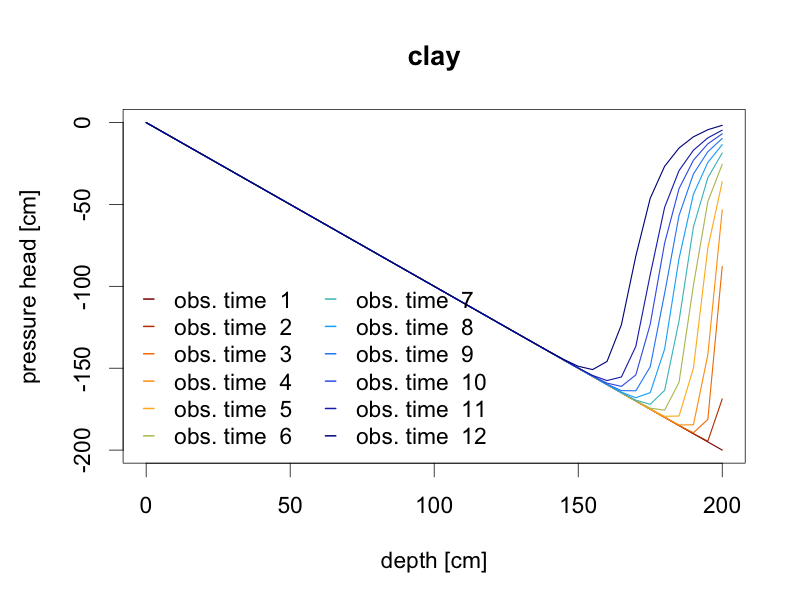
\includegraphics[width=0.49\textwidth]{Fig_inf1/obs_press_head_clay.png}
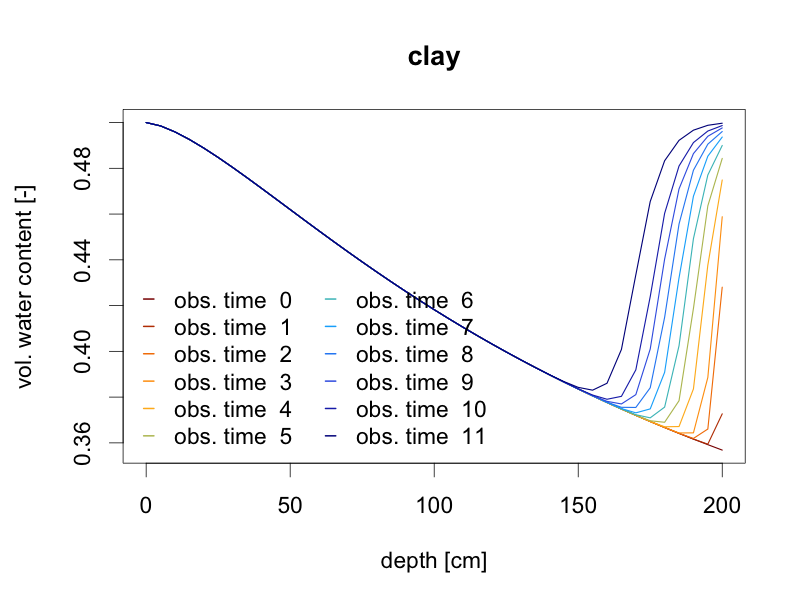
\includegraphics[width=0.49\textwidth]{Fig_inf1/obs_water_clay.png}
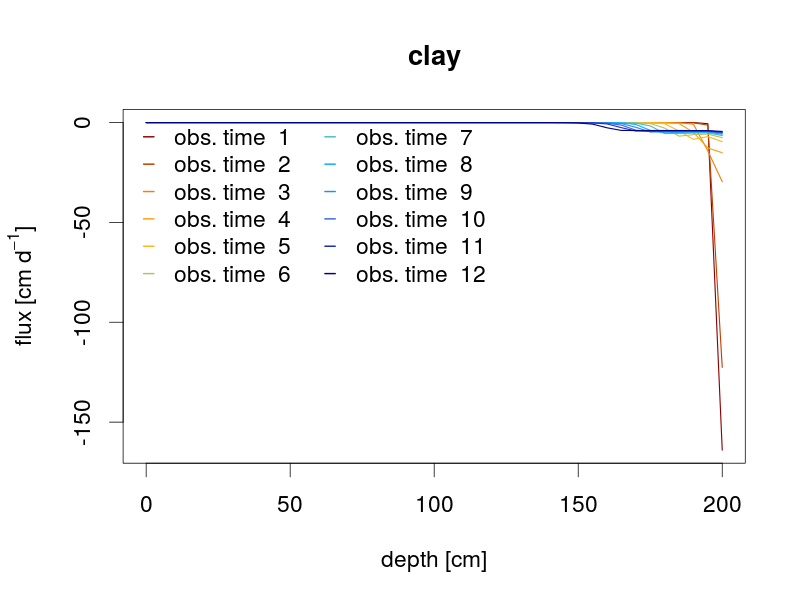
\includegraphics[width=0.49\textwidth]{Fig_inf1/obs_flux_clay.png}
\caption{Observation time series of pressure head, vol. water content and flux of infiltration into clay.}

\end{figure}

\newpage
\newpage
\newpage
\newpage
\subsection{Outcome}
\begin{enumerate}
\item You got familiar with the $DRUtES$ standard Richards Equation modules in 1D.
\item You understand basic parameterization of a typical sand, silt and clay with the van Genuchten-Mualem model.
\item You simulated infiltration in different soils.
\item You understand the term \emph{Neumann boundary condition} and \emph{initial condition}.
\item You understand the effects of different discretizations.
\end{enumerate}
